\section{Implementing Linear Regression with \texttt{Python}}

Let us move forward and build a practical simple linear regression model, examining the empirical challenges we face and how they can be addressed to make our model more robust.

We will use the advertising expenditure dataset analyzed earlier.

The following two primary libraries implement linear regression models in \texttt{Python}:
\begin{itemize}
	\item The \texttt{ols} method (Ordinary Least Squares) within \texttt{statsmodels.formula.api}.
	\item The \texttt{scikit-learn} machine learning package.
\end{itemize}

Let us implement a simple linear regression model using the first method and subsequently expand it into a multiple linear regression model. Afterwards, we will also examine how the second method (\texttt{scikit-learn}) is utilized to achieve the same objectives.

\subsection{Linear Regression Using \texttt{statsmodels}}
\lstinputlisting[language=Python]{../code/regresion/statsModelExample.py}

Recall that this dataset contains historical information regarding advertising budgets allocated to TV, radio, and newspaper campaigns for particular consumer products, along with the resulting sales figures.

We naturally anticipate a positive correlation between these advertising budgets and overall sales volume. Indeed, we previously verified that a strong positive correlation exists between TV advertising expenditures and sales.

Let us now explore this relationship explicitly using the following Python code:
\begin{lstlisting}[language=Python]
import statsmodels.formula.api as smf
model1 = smf.ols(formula='Sales~TV', data=advert).fit()
print(model1.params)
\end{lstlisting}

From this execution, we obtain the following parameter output:
\begin{lstlisting}[language=Python]
Intercept    7.032594
TV           0.047537
dtype: float64
\end{lstlisting}

Here, we have assumed that a linear regression relationship links TV advertising expenditures to product sales, and we have determined the line of best fit using the Ordinary Least Squares optimization method. In our formal mathematical notation, these estimated regression parameters correspond to:
\begin{align}
	\a = 7.032594, \quad \beta = 0.047537
\end{align}
and the resulting empirical equation for our predictive model is:
\begin{align}
	\texttt{Sales} = 7.032 + 0.047 \times \texttt{TV}
\end{align}

As we established theoretically, these parameter estimates are accompanied by statistical hypothesis tests and associated $p$-values. \emph{If these $p$-values are sufficiently small, we reject the null hypothesis and accept that these parameters are significantly different from zero, confirming their statistical significance within the model.}

Let us inspect the exact $p$-values associated with our estimated coefficients:
\begin{lstlisting}[language=Python]
print(model1.pvalues)

Intercept    1.406300e-35
TV           1.467390e-42
dtype: float64
\end{lstlisting}

As can be observed, these $p$-values are virtually zero; therefore, both parameters are highly statistically significant.

Let us next examine another crucial indicator of model performance: the coefficient of determination, $R^2$. Although we previously computed it manually from scratch, we can retrieve it directly from our fitted model object using the following line of code:
\begin{lstlisting}[language=Python]
print(model1.rsquared)

0.61187505085
\end{lstlisting}

If we require a comprehensive overview of all statistical parameters, diagnostic tests, and model metrics in a single step, we can invoke the summary method:
\begin{lstlisting}[language=Python]
print(model1.summary())
\end{lstlisting}

Which yields the following complete statistical table:
\begin{lstlisting}[language=Python]
OLS Regression Results
==============================================================================
Dep. Variable:                  Sales   R-squared:                       0.612
Model:                            OLS   Adj. R-squared:                  0.610
Method:                 Least Squares   F-statistic:                     312.1
Date:                Sun, 29 Oct 2017   Prob (F-statistic):           1.47e-42
Time:                        04:11:12   Log-Likelihood:                -519.05
No. Observations:                 200   AIC:                             1042.
Df Residuals:                     198   BIC:                             1049.
Df Model:                           1
Covariance Type:            nonrobust
==============================================================================
                 coef    std err          t      P>|t|      [0.025      0.975]
------------------------------------------------------------------------------
Intercept      7.0326      0.458     15.360      0.000       6.130       7.935
TV             0.0475      0.003     17.668      0.000       0.042       0.053
==============================================================================
Omnibus:                        0.531   Durbin-Watson:                   1.935
Prob(Omnibus):                  0.767   Jarque-Bera (JB):                0.669
Skew:                          -0.089   Prob(JB):                        0.716
Kurtosis:                       2.779   Cond. No.                         338.
==============================================================================
\end{lstlisting}

As we can observe, the overall $F$-statistic for this simple regression model is extremely large ($312.1$), and its corresponding $p$-value (`Prob (F-statistic)`) is negligible ($1.47\times 10^{-42}$), which confirms that our parameter estimates provide statistically significant predictive utility.

Now let us predict sales values directly from our estimated linear regression equation using the `predict` method:
\begin{lstlisting}[language=Python]
sales_pred = model1.predict(pd.DataFrame(advert['TV']))
print(sales_pred.head())

0    17.970775
1     9.147974
2     7.850224
3    14.234395
4    15.627218
dtype: float64
\end{lstlisting}

This method systematically evaluates our fitted model equation for each observational row using its specific \texttt{TV} expenditure entry.

We can plot \texttt{sales\_pred} against the actual \texttt{TV} advertising expenditure to visualize the fitted line of best fit:
\begin{lstlisting}[language=Python]
import matplotlib.pyplot as plt
advert.plot(kind='scatter', x='TV', y='Sales')
plt.plot(pd.DataFrame(advert['TV']), sales_pred, c='red', linewidth=2)
plt.show()
\end{lstlisting}

\begin{center}
	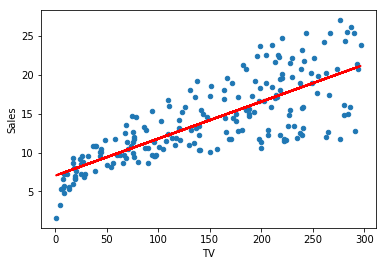
\includegraphics[width=10cm,keepaspectratio=true]{./images/statsModelExample.png}
\end{center}

Now let us compute the exact Residual Standard Error (\texttt{RSE}):
\begin{lstlisting}[language=Python]
advert['sales_pred'] = 0.047537 * advert['TV'] + 7.03
advert['RSE'] = (advert['Sales'] - advert['sales_pred']) ** 2
SSD = advert.sum()['RSE']
n = len(advert["Sales"])
RSE = np.sqrt(SSD / (n - 2))
salesmean = np.mean(advert['Sales'])
error = RSE / salesmean
print(RSE, salesmean, error)
\end{lstlisting}

This output displays three numerical values: the first is $\texttt{RSE} \approx 3.25$, the second is $\texttt{salesmean}$ (the arithmetic mean of actual sales) $\approx 14.02$, and the third ($\texttt{error}$) represents their ratio, which equals approximately $0.23$.

Therefore, on average, predictions yielded by this model exhibit an inherent discrepancy of roughly $23\%$, even assuming the regression coefficients are precisely estimated.

This represents a notable margin of prediction error that we would like to reduce. Furthermore, the baseline $R^2 = 0.61$ leaves substantial room for improvement.

A natural logical next step is to incorporate additional predictor columns into our model to determine whether capturing multi-channel marketing dynamics improves overall predictive accuracy.
